The \texttt{\pkglnk{model.library}} contains classes representing the different libraries provided by the application.
Each library consists of a collection of commonly needed \texttt{\hyperref[type:edu.kit.wavelength.client.model.term.LambdaTerm]{LambdaTerm}}s and corresponding names used to reference them.
After enabling a library  these names can be used in place of the longer and more difficult to work with terms.

The \texttt{\lnk{Boolean}} library contains the terms representing the boolean values "true" and "false".

The \texttt{\lnk{TuplesAndLists}} library contains the terms implementing tuples and lists and the functions needed to work with them.

The \texttt{\lnk{NaturalNumbers}} library contains the church encodings of the natural numbers and terms implementing basic arithmic functions.

The \texttt{\lnk{YCombinator}} library contains the Y combinator making recursive function calls possible.

All libraries implement the \texttt{\lnk{Library}} interface allowing the application to be expanded with more libraries provided they too implement this interface.

The library classes are used by the \texttt{\hyperref[type:edu.kit.wavelength.client.model.term.parsing.Parser]{Parser}} 
to access the terms belonging to names in the input String. 
After it has been successfully parsed each used library term is represented by a
\texttt{\hyperref[type:edu.kit.wavelength.client.model.term.NamedTerm]{NamedTerm}} 
in the \texttt{\hyperref[type:edu.kit.wavelength.client.model.term.LambdaTerm]{LambdaTerm}} object structure.

\begin{figure}[H]
	\centering
	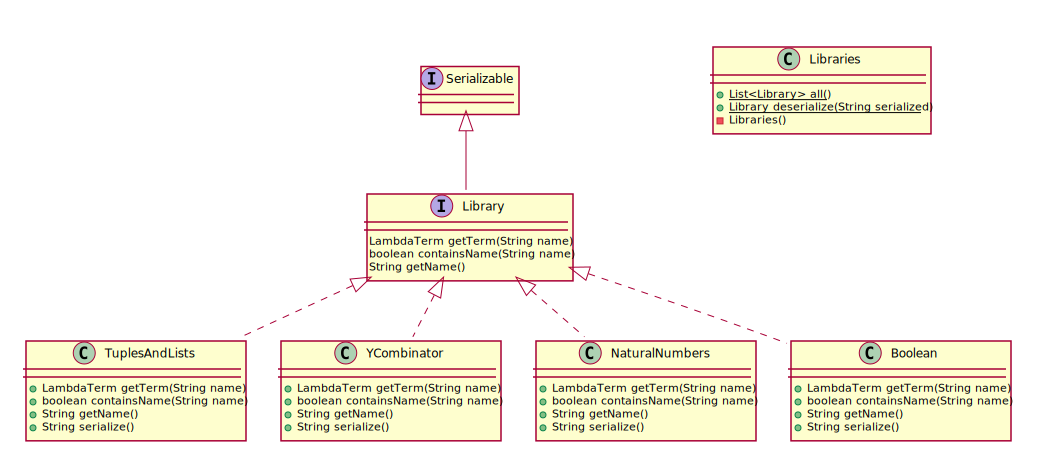
\includegraphics[width=\textwidth]{packageDiagrams/libraryPackage}
\end{figure}